\section{Dynamic Adaptive Streaming over HTTP}
\begin{figure}[!t]
	\centering
	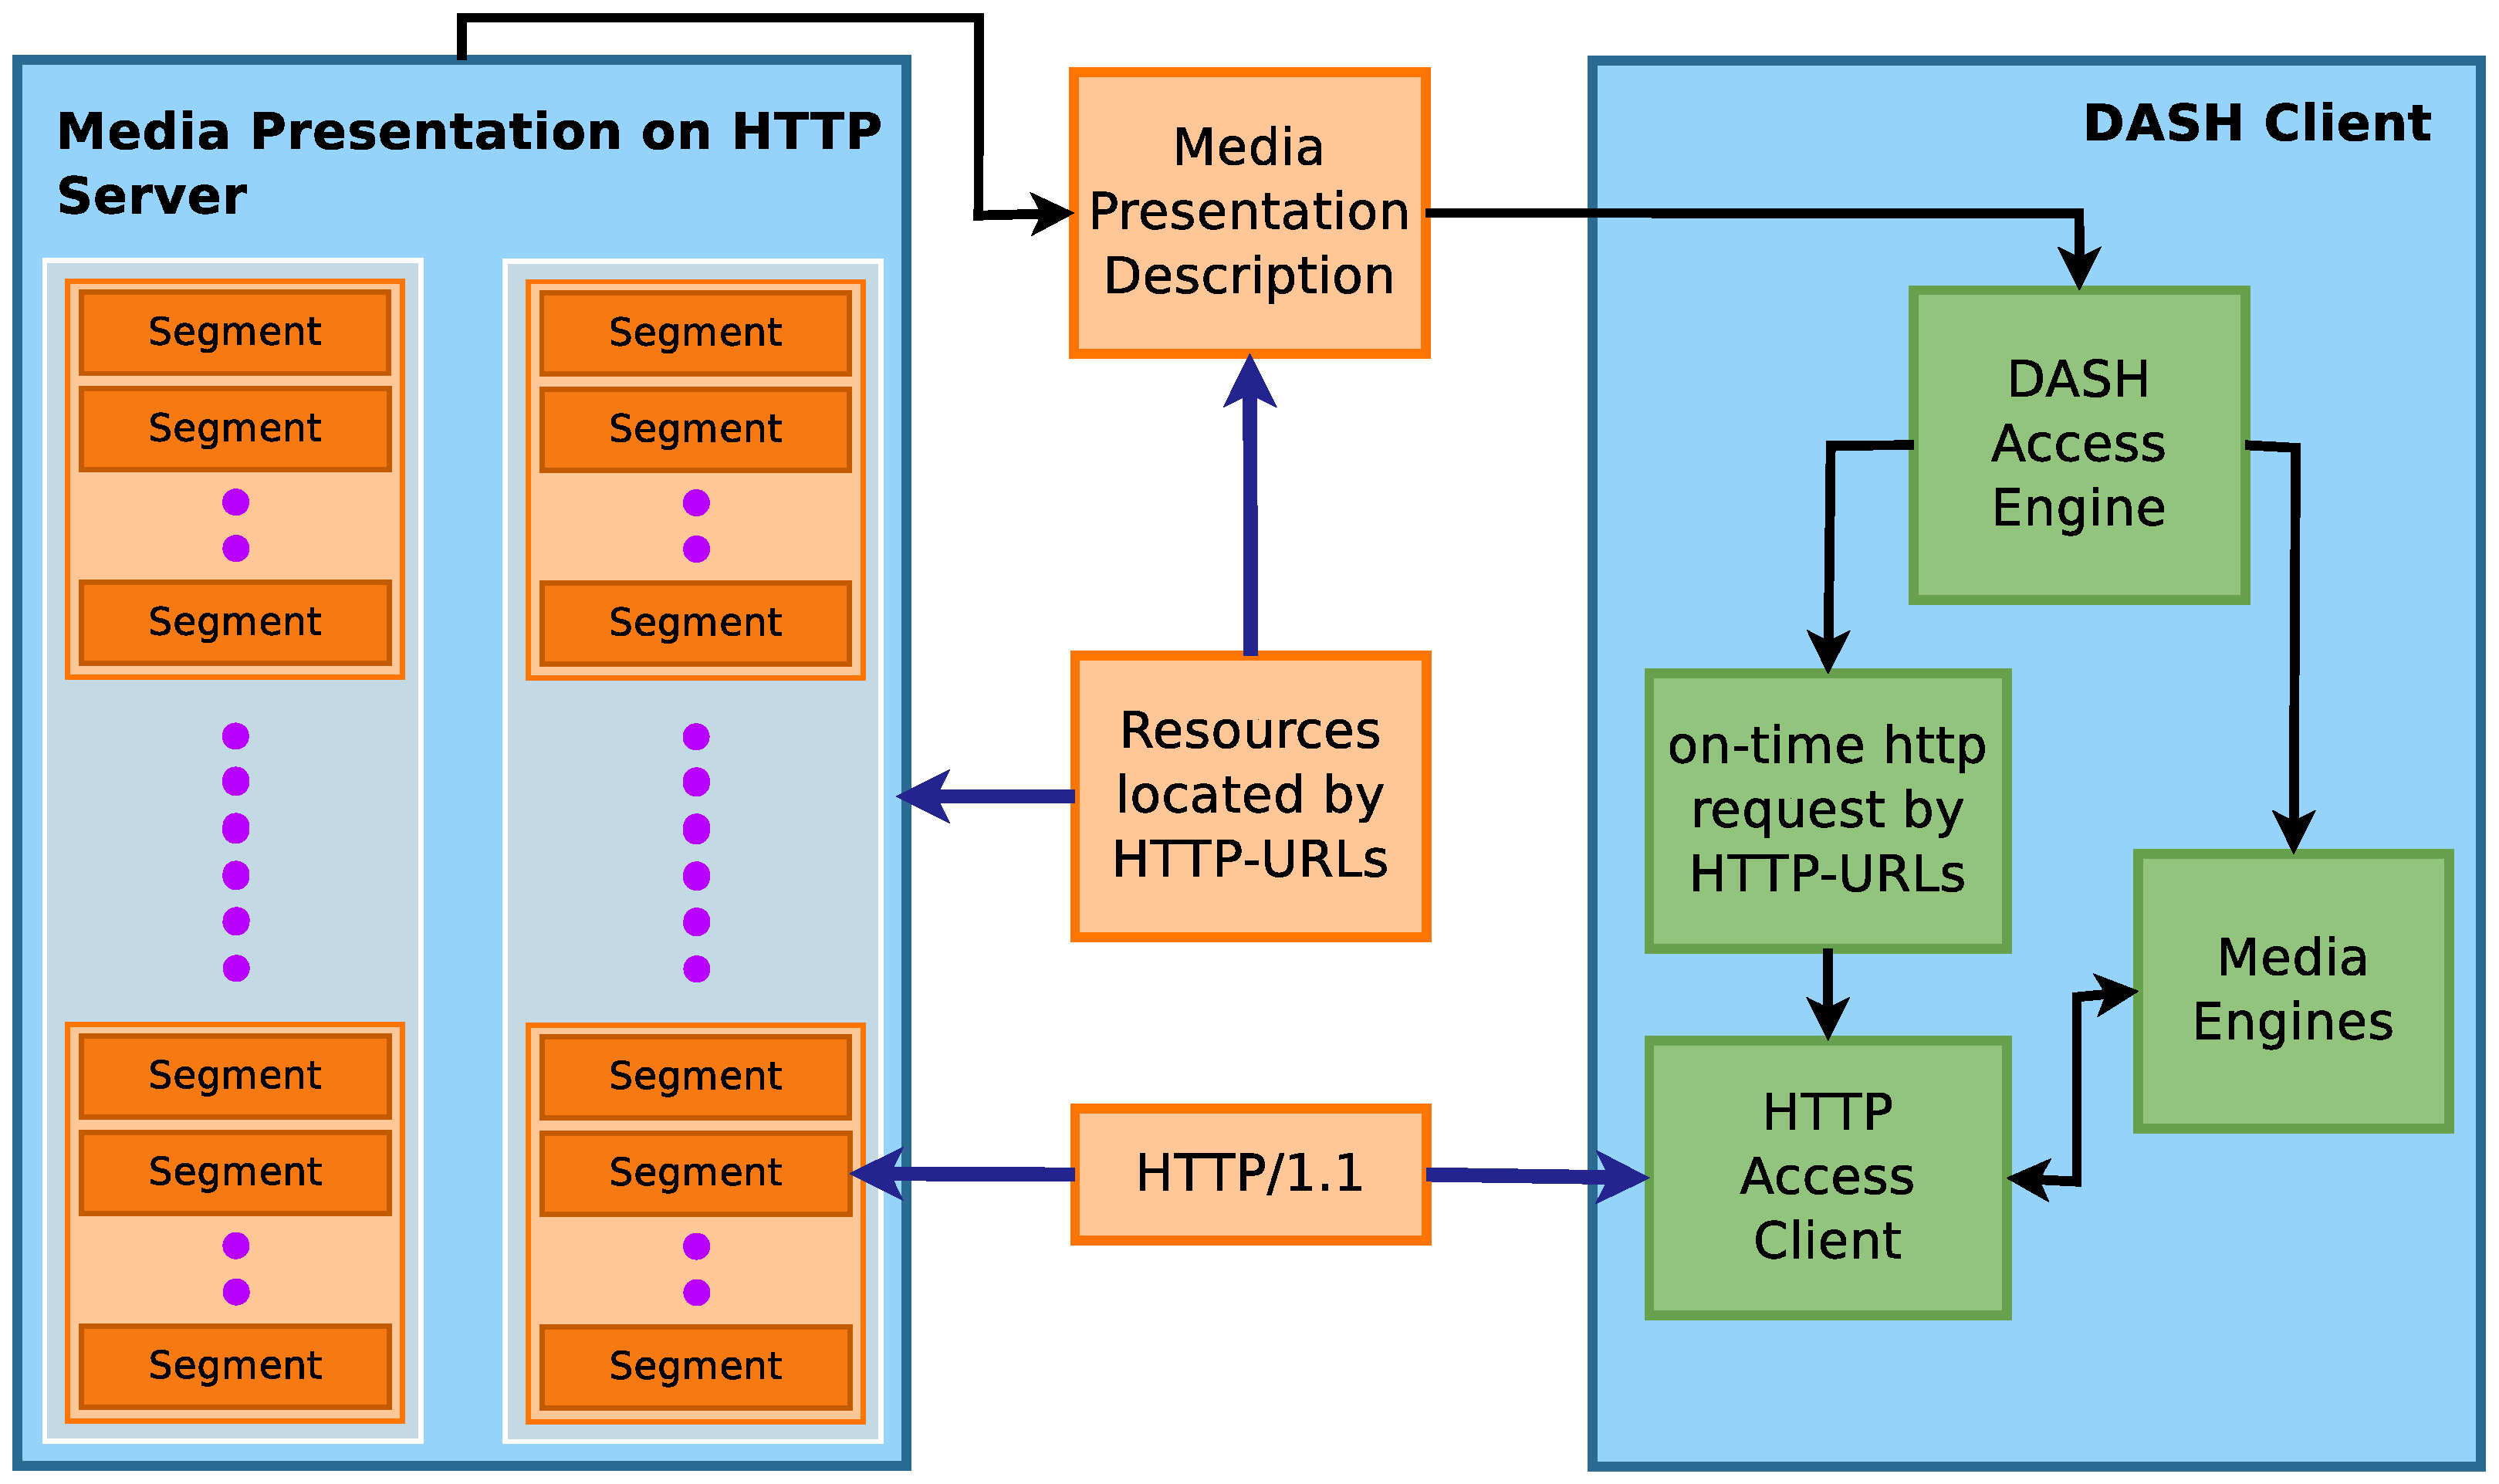
\includegraphics[scale=0.25]{img/dash-arch}
	\caption{\small{DASH Architecture -- On the left side, the server-side media storage is shown, where content is divided into small segments of alternative bitrates. On the right side, the DASH client architecture is shown; the {\it DASH Access Engine} monitors the network bandwidth at the client and accordingly decides which segment to request from the server. (Image Source: https://www.w3.org/2011/09/webtv/slides/W3C-Workshop.pdf) (accessed: \today)}}
	\label{fig:dash}
\end{figure}
In 2009, Apple developed the HTTP Live Streaming (HLS) to replace the existing Real Time Streaming Protocol (RTSP)-based video delivery for its QuickTime live streaming server\footnote{\url{https://appleinsider.com/articles/09/07/08/apple_launches_http_live_streaming_standard_in_iphone_3_0.html} (accessed: \today)}. Dynamic Adaptive Streaming over HTTP (DASH), sometimes calls as MPEG-DASH, is a technology developed under MPEG to stream videos over HTTP. MPEG started working for DASH in 2010 and standardized it in 2011~\cite{ISO/IEC23009-1:2019}. After the release of {\tt dash.js} by DASH Industry Forum (DASH-IF), almost all the streaming services, including YouTube, NetFlix, Samsung, etc., adopt DASH in their services.

\fig{\ref{fig:dash}} shows the broad architecture of DASH. Video streaming using DASH is a two-step procedure: a) preprocessing of the video files to distribute, and b) the streaming. 


\subsubsection{Video Preprocessing}
In the preprocessing (we also call it DASHifying) step, a streaming provider prepares the required files. It first splits the audio and video streams and encodes them into multiple bitrate versions. At this phase, the encoder needs to ensure that it aligns the I-frames\footnote{I-frame: a special type of frame that contains a complete picture and no-other frame required to render it. More details: \url{https://en.wikipedia.org/wiki/Video_compression_picture_types} (accessed: \today)} across different bitrate versions and places all the metadata at the beginning of the file. After encoding, three different types of files are created from the streams. These files are i) media index files, ii) media data files, and iii) a media presentation description file.

{\bf Media Index Files:} In general, when any media data is stored in a file, the file contains two pieces of information, a) the initialization part and b) the encoded media data. The initialization part contains information to decode the encoded data, which is the index for the original media data. The DASH mandates that this initialization data should be stored in a separate file. So, while encoding a video into different bitrate versions, the metadata part needs to be kept at the starting of the output file. The index files are usually smaller than any of the media data, so it does not pose any overhead to the system.

{\bf Media Data Files:} The media data file contains the encoded media. According to DASH, media data are segmented into multiple chunks with equal playback time. All the segments should have an I-frame at the beginning of the chunk.

{\bf Media Presentation Description (MPD):} It is an {\tt XML} file that contains the metadata required to stream the video. It lists the different audio and video qualities available for streaming and the URLs for the media index and media data. It also contains the codec, bitrate, and playback duration of individual chunks for each quality.

The preprocessing phase ends after storing all these different files in an HTTP(S) file server. DASH does not require anything else on the server-side to stream a video. This is valid for both VoD and live streaming. However, in live streaming, the segments are created on-the-fly and placed in the server before any client requests it.

\subsubsection{Video Streaming}
The second phase of the DASH-based streaming is the video streaming. DASH requires a smart player that can understand DASH and play the video. Any DASH-based video streaming starts by downloading the MPD file. The player reads the MPD file to get information regarding the video.  At this point, the player has to decide which quality it wants to play based on the ABR algorithm running inside the player, and then it fetches the video chunks in the preferred quality. DASH offloads the entire decision to the player so that any existing content delivery network can stream the video content. There are instances where media index files and media data are not chunked, instead kept in a fixed file. While this saves lot of disk space, the server has to support the HTTP range-request\footnote{\url{https://developer.mozilla.org/en-US/docs/Web/HTTP/Range_requests} (accessed: \today)}, and the player can get the desired chunk using the {\tt range} header.

DASH also allows streaming providers to support various client platforms, encodes video in various codec and puts all the information in the MPD file. Although the size of the MPD file can be large, the player can choose a platform supported codec and play it without any hassle.


\subsection{Adaptive Bitrate Algorithms}
The adaptive bitrate algorithms are the heart of the DASH-based streaming system as it decides the quality of every video segment on-the-fly. By default, the ABR algorithm runs just before fetching the next video segment to be downloaded. As the ABR algorithm is a part of the player, it has access to all the playback related parameters, and it can use any of those parameters to decide quality for the next chunk. The primary goal of any ABR algorithm is to maximize the Quality of Experience (QoE) so that users can enjoy the streaming.

\subsubsection{Quality of Experience (QoE)}
QoE is a crucial parameter in any field which involves end-users. In the case of video streaming, QoE is a metric to measure whether the user has enjoyed the video or not during the streaming. QoE is mostly a metric of user perspective, and it depends on several factors such as the video startup delay, quality fluctuations, the overall quality, rebuffering, audio/video device, and video content. Although all these parameters are essential, it is not easy to measure user-dependent parameters and video content. Several researchers tried to design the best measurable metric to calculate the QoE, which can be acceptable. Mok \etal \cite{5990550} tried to estimate QoE from the network QoS. They suggested that the user QoS (or QoS of HTTP) is the QoE. Various researches like \cite{10.1145/2155555.2155558,10.1145/3394171.3413512} tried to use Peak Noise to Signal Ratio (PSNR) and Structural Similarity Index Measurement (SSIM) as a parameter for QoE. Spiteri \etal\ considered only the rebuffering and the average quality as the QoE in their ABR algorithm BOLA~\cite{Spiteri2016}. Yin \etal~\cite{yin2015control} proposed an equation (\eqn{\ref{eqn:QoE}}) to calculate the QoE using four parameters:
\begin{itemize}
	\item {\bf Video Startup Delay,} which is the delay before the playback can be started. In the case of ABR-based solution, the startup delay depends on the efficient initial quality selection. Most of the ABR algorithms ignore this parameter and set the initial quality as the lowest video quality available.
	\item {\bf Quality:} The sharpness of the video determines the quality of the video or audio. The sharpness of a video is directly related to the bitrate. It is expected that sharp media has better media details in both audio and video, thus providing a better experience in enjoying the stream. Any ABR tries to maintain the bitrate as high as possible so that the QoE improves.
	\item {\bf Smoothness:} DASH allows the player to change the video quality on-the-fly. Frequent quality updates disrupt the smoothness of the video watching experience. So, ABR needs to minimize the quality change during playback.
	\item {\bf Rebuffering:} Rebuffering is the most irritating experience for any user. The entire DASH and DASH like system is developed to minimize rebuffering during the video playback. The outmost responsibility of any ABR algorithm is to minimize the rebuffering by selecting appropriate video quality, based of the current network quality.
\end{itemize}
\begin{equation}
\label{eqn:QoE}
QoE = \sum_{i=1}^N q(R_i) - \lambda\sum_{i=1}^{N-1}\left|q(R_{i+1})-q(R_i) - \mu\sum_{i=1}^N \delta_i - \mu_s T_s\right|
\end{equation}
\eqn{\ref{eqn:QoE}} is used by most modern ABR algorithms which measure the QoE for a video with $N$ segments, where $R_i$ represents the bitrate of $i^{th}$ segment, $q(.)$ is the utility function, $\delta_i$ is the stall before the $i^{th}$ segment ($\delta_0$ is always zero), $T_s$ is the startup delay. $\lambda$, $\mu$ and $\mu_s$ are constant weights to define importance of individual parameters.

To enhanced the online streaming experience, researchers have developed various systems and ABR algorithms. We categorize the ABR algorithms broadly in a) classical ABR algorithms and b) learning based ABR algorithms. In the following sections, we discuss both of these ABR algorithms. Finally, we discuss the ABR algorithms specially designed for live streaming and smartphones.

